% Homogenization benchmark report -- compile with tectonic (or pdflatex twice).
\documentclass[11pt]{article}
\usepackage[margin=1in]{geometry}
\usepackage{amsmath,amssymb,bm}
\usepackage{graphicx}
\usepackage{booktabs}
\usepackage{siunitx}
\usepackage[table]{xcolor}
\usepackage[hidelinks]{hyperref}
\usepackage{caption}
\usepackage{placeins}
\graphicspath{{figures/}}
\newcommand{\T}{^{\mathsf{T}}}

\title{\textbf{Homogenization benchmark of thin-walled MSG shell models\\
(Reissner--Mindlin and Kirchhoff) against 3D solid finite elements:\\
isotropic and $[45/\!-\!45]$ tubes and plate-strips, thin to thick}}
\author{Akshat Bagla\\\small School of Aeronautics and Astronautics, Purdue University%
\thanks{Author/affiliation placeholder --- verify before distribution.}}
\date{\today}

\begin{document}
\maketitle

\begin{abstract}
We benchmark a thin-walled Mechanics-of-Structure-Genome (MSG) shell
cross-sectional analysis---in both Reissner--Mindlin (RM, $C^0$) and Kirchhoff
($C^1$) wall kinematics---against a 3D solid finite-element cross-sectional
analysis (FEniCSx), which here plays the role of VABS. Four sections are studied
across a thin-to-thick sweep: a \emph{closed} circular tube and an \emph{open}
flat plate-strip, each isotropic and balanced anisotropic $[45/\!-\!45]$. The
report is results-focused: it reports the full Timoshenko $6\times6$ stiffness
for every case, term by term, with the matrix components labelled by both index
and engineering meaning ($C_{11}{=}EA$, $C_{22}{=}GA_2$, $C_{33}{=}GA_3$,
$C_{44}{=}GJ$, $C_{55}{=}EI_2$, $C_{66}{=}EI_3$).
\emph{Key results.} For the \textbf{tube}, both shell models reproduce the solid
to $<1\%$ on every non-zero stiffness at the mid-surface reference across the
whole range ($h/R=0.01$--$0.20$); the outer-mould-line (OML) reference adds an
$O(h/R)$ curvature/arc-length drift. For the \textbf{strip}, the axial $EA$ and
the strong in-plane bending $EI_3$ are exact in both models; the open section
proved a discriminating test for torsion: it exposed (and we corrected) the RM
twist measure, which must carry the full $\kappa_{12}{+}\kappa_{21}{=}{-}2\kappa_1$.
With the correction the RM torsion recovers the St-Venant value exactly and
\emph{outperforms} Kirchhoff for the thick open section ($GJ$ at $h/W{=}0.20$: RM
$-0.1\%$ vs.\ KF $+22\%$). The weak bending $EI_2$ is captured at the centre
(Kirchhoff marginally better; RM slightly soft owing to bend--twist coupling).
The transverse shear $GA$ is the genuinely method-sensitive quantity: the
thickness-direction $GA_3$ of a wide strip is a two-dimensional, $h^3$-governed
field that no 1D-shell genome resolves (both models err), and the in-plane $GA_2$
of the balanced strip is carried by Kirchhoff but under-predicted by the RM $C^0$
kinematics. The off-diagonal couplings confirm the theory: $C_{15},C_{16},C_{56}$
are identically zero at the centroid for these symmetric sections (appearing only
as a parallel-axis artifact under an off-centroid reference), while the genuine
antisymmetric-$[45/\!-\!45]$ couplings are extension--twist ($C_{14}$) and
transverse-shear--bending ($C_{25}/C_{36}$).
\end{abstract}

%================================================================
\section{Setup}
\paragraph{Sections and materials.} Tube radius $R=1$~m, strip width $W=1$~m;
wall/laminate thickness swept over $h/R$ (resp.\ $h/W$)
$=\{0.01,0.03,0.06,0.12,0.20\}$. Isotropic: $E=\SI{70}{GPa}$, $\nu=0.3$
($G=\SI{26.923}{GPa}$). Anisotropic $[45/\!-\!45]$: $E_1=37$, $E_2=E_3=9$,
$G_{ij}=4$~GPa, $\nu=0.3$; the $+45^\circ$ ply is the outer (tube) / top (strip)
band and $-45^\circ$ the inner / bottom band. The shell wall is referenced at the
mid-surface (\emph{centre}, $\mathrm{frac}=0.5$) or the outer mould line
(\emph{OML}, $\mathrm{frac}=0$).

\paragraph{Models.} \emph{Solid} --- 2D solid cross-sectional analysis (FEniCSx,
first-order quadrilaterals, full 3D constitutive, lamina baked into the element
frame); $N_c=200{\times}N_r=16$ (tube) and $120{\times}16$ (strip), $8$ elements
per ply for $[45/\!-\!45]$. \emph{Shell} --- the 1D MSG structure genome along the
wall with the $8\times8$ plate law
$\{\bm N,\bm M,\bm Q\}=[\,\mathbf A,\mathbf B,\bm0;\mathbf B,\mathbf D,\bm0;
\bm0,\bm0,\bm G\,]\{\bm\varepsilon^0,\bm\kappa,\bm\gamma^s\}$ condensed to the
Timoshenko $6\times6$, in two kinematics: Kirchhoff ($C^1$ Hermite, no transverse
shear) and Reissner--Mindlin ($C^0$ Lagrange, transverse shear retained). The
geometry, $[45/\!-\!45]$ orientation, and the matching solid mesh are shown in
Figs.~\ref{fig:geom_tube}--\ref{fig:geom_strip}; the closed tube uses connectivity
that wraps, the open strip does not.

\begin{figure}[t]\centering
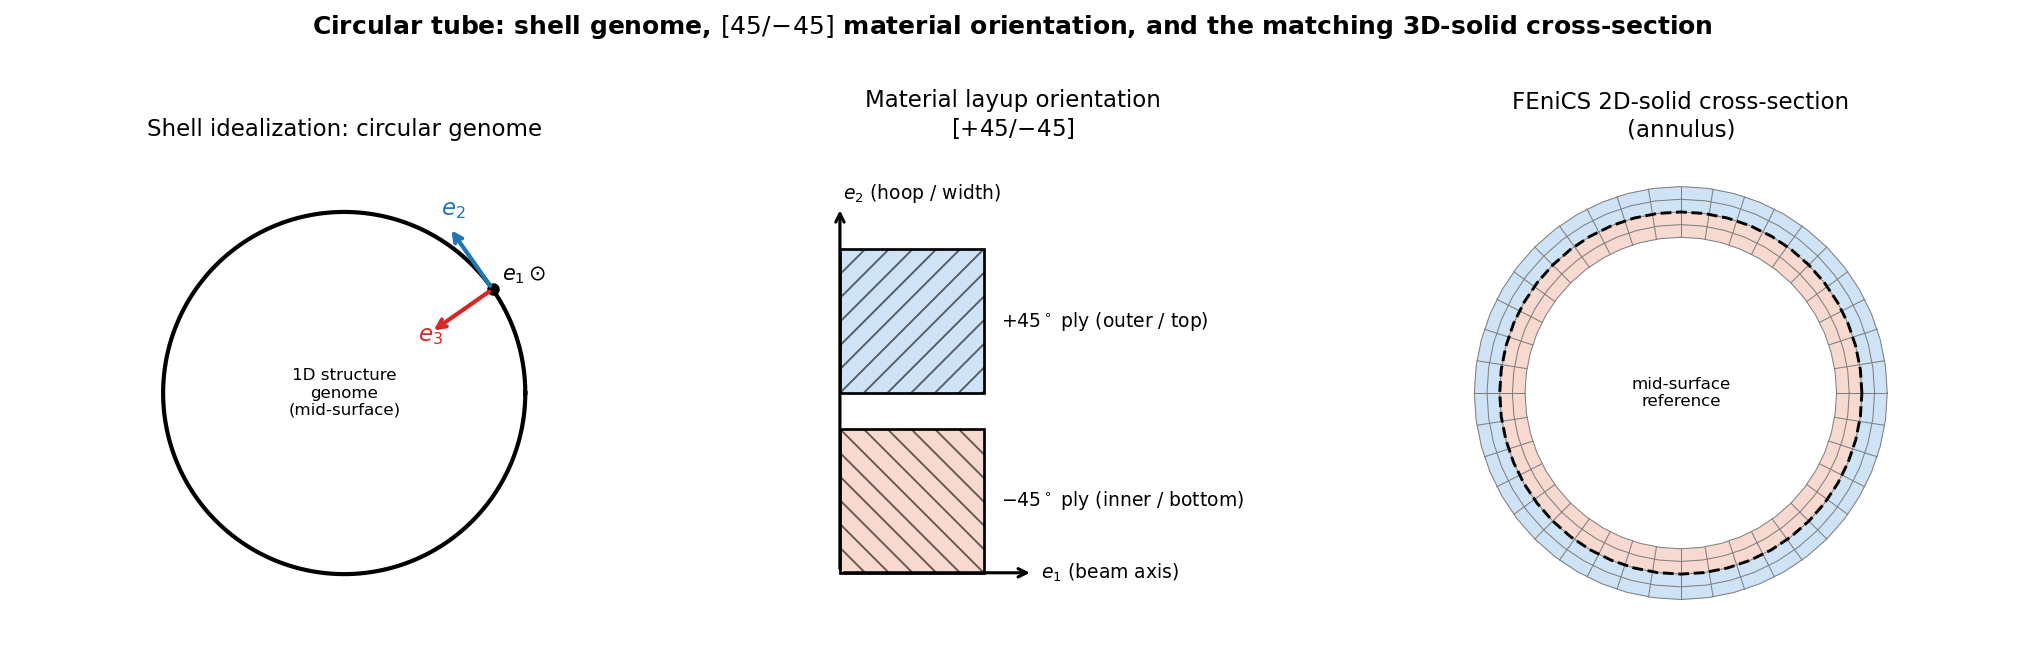
\includegraphics[width=\textwidth]{geom_tube.png}
\caption{\textbf{Tube.} Left: the 1D shell genome (mid-surface circle) with the
local frame $e_1$ (beam, out of plane), $e_2$ (hoop), $e_3$ (through-thickness).
Centre: the $[+45/\!-\!45]$ material orientation (fiber tows shown in each ply,
relative to $e_1$/$e_2$). Right: the matching FEniCS 2D-solid annulus with the
two ply bands and the mid-surface reference.}
\label{fig:geom_tube}
\end{figure}

\begin{figure}[t]\centering
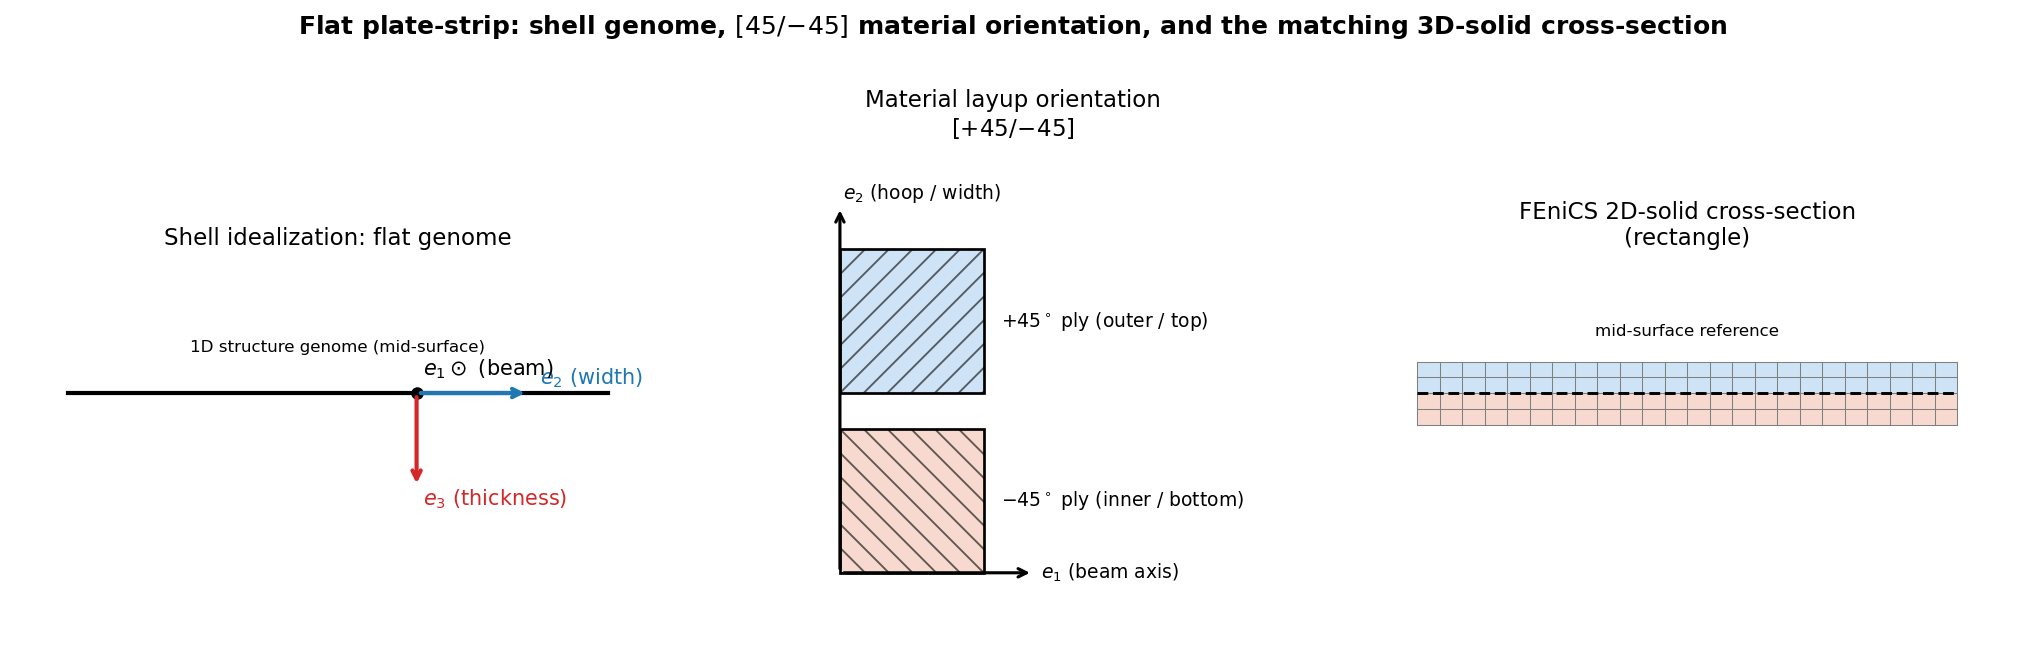
\includegraphics[width=\textwidth]{geom_strip.png}
\caption{\textbf{Plate-strip.} Left: the flat 1D genome with the local frame
($e_2$ along the width, $e_3$ through the thickness). Centre: the same
$[+45/\!-\!45]$ orientation. Right: the matching FEniCS 2D-solid rectangle. The
strip is an \emph{open} section (free edges), unlike the closed tube.}
\label{fig:geom_strip}
\end{figure}

%================================================================
\section{Results}

\subsection{Circular tube (closed section)}
At the \textbf{centre} reference the shell is essentially exact on the full
$6\times6$: $EA$ within $0.1\%$ and $GA$, $GJ$, $EI$ within $\approx1\%$ even at
$h/R=0.20$, for \emph{both} RM and Kirchhoff (Fig.~\ref{fig:err_tube_iso},
\ref{fig:err_tube_aniso}; Tables~\ref{tab:tube_iso_props}--\ref{tab:tube_aniso_full}).
The balanced $[45/\!-\!45]$ tube shows the expected high torsional stiffness
($GJ/EA\approx0.85$), captured to $<1\%$. At the \textbf{OML} reference the error
grows almost linearly in $h/R$: $EA$, $EI$ over-predict by $\approx h/2R$ (the
$(1+z/R)$ curvature/arc-length factor) and $GA$, $GJ$ pick up an $O(h/R)$ drift.
The off-diagonal couplings are negligible for these symmetric / balanced sections
(see the full $6\times6$, Tables~\ref{tab:tube_iso_full},
\ref{tab:tube_aniso_full}).

\begin{figure}[t]\centering
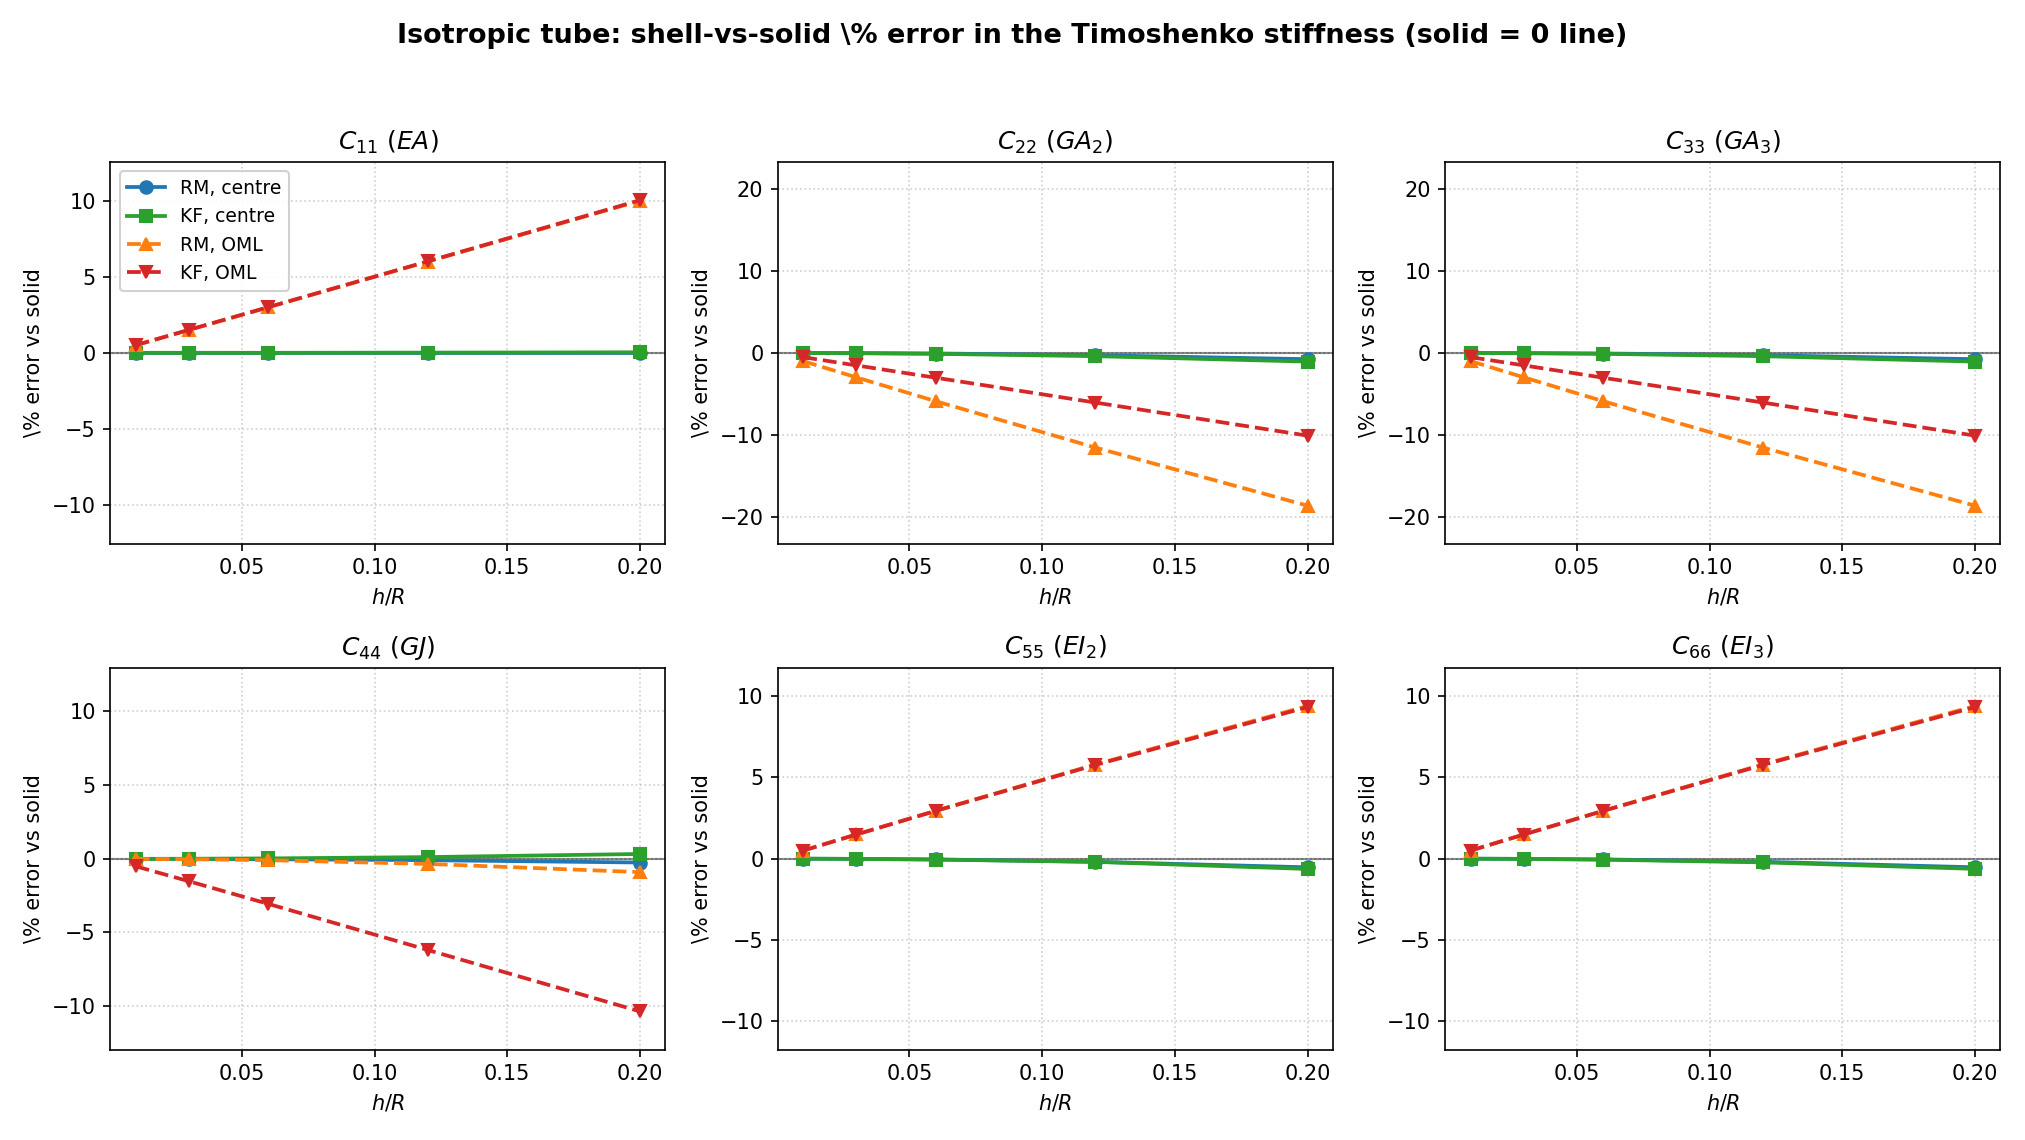
\includegraphics[width=0.96\textwidth]{err_tube_iso.png}
\caption{Isotropic tube: \% error vs.\ the solid for each Timoshenko component.
Centre-reference curves (solid lines) hug zero through the thick range; OML
(dashed) drifts $O(h/R)$.}
\label{fig:err_tube_iso}
\end{figure}

\begin{figure}[t]\centering
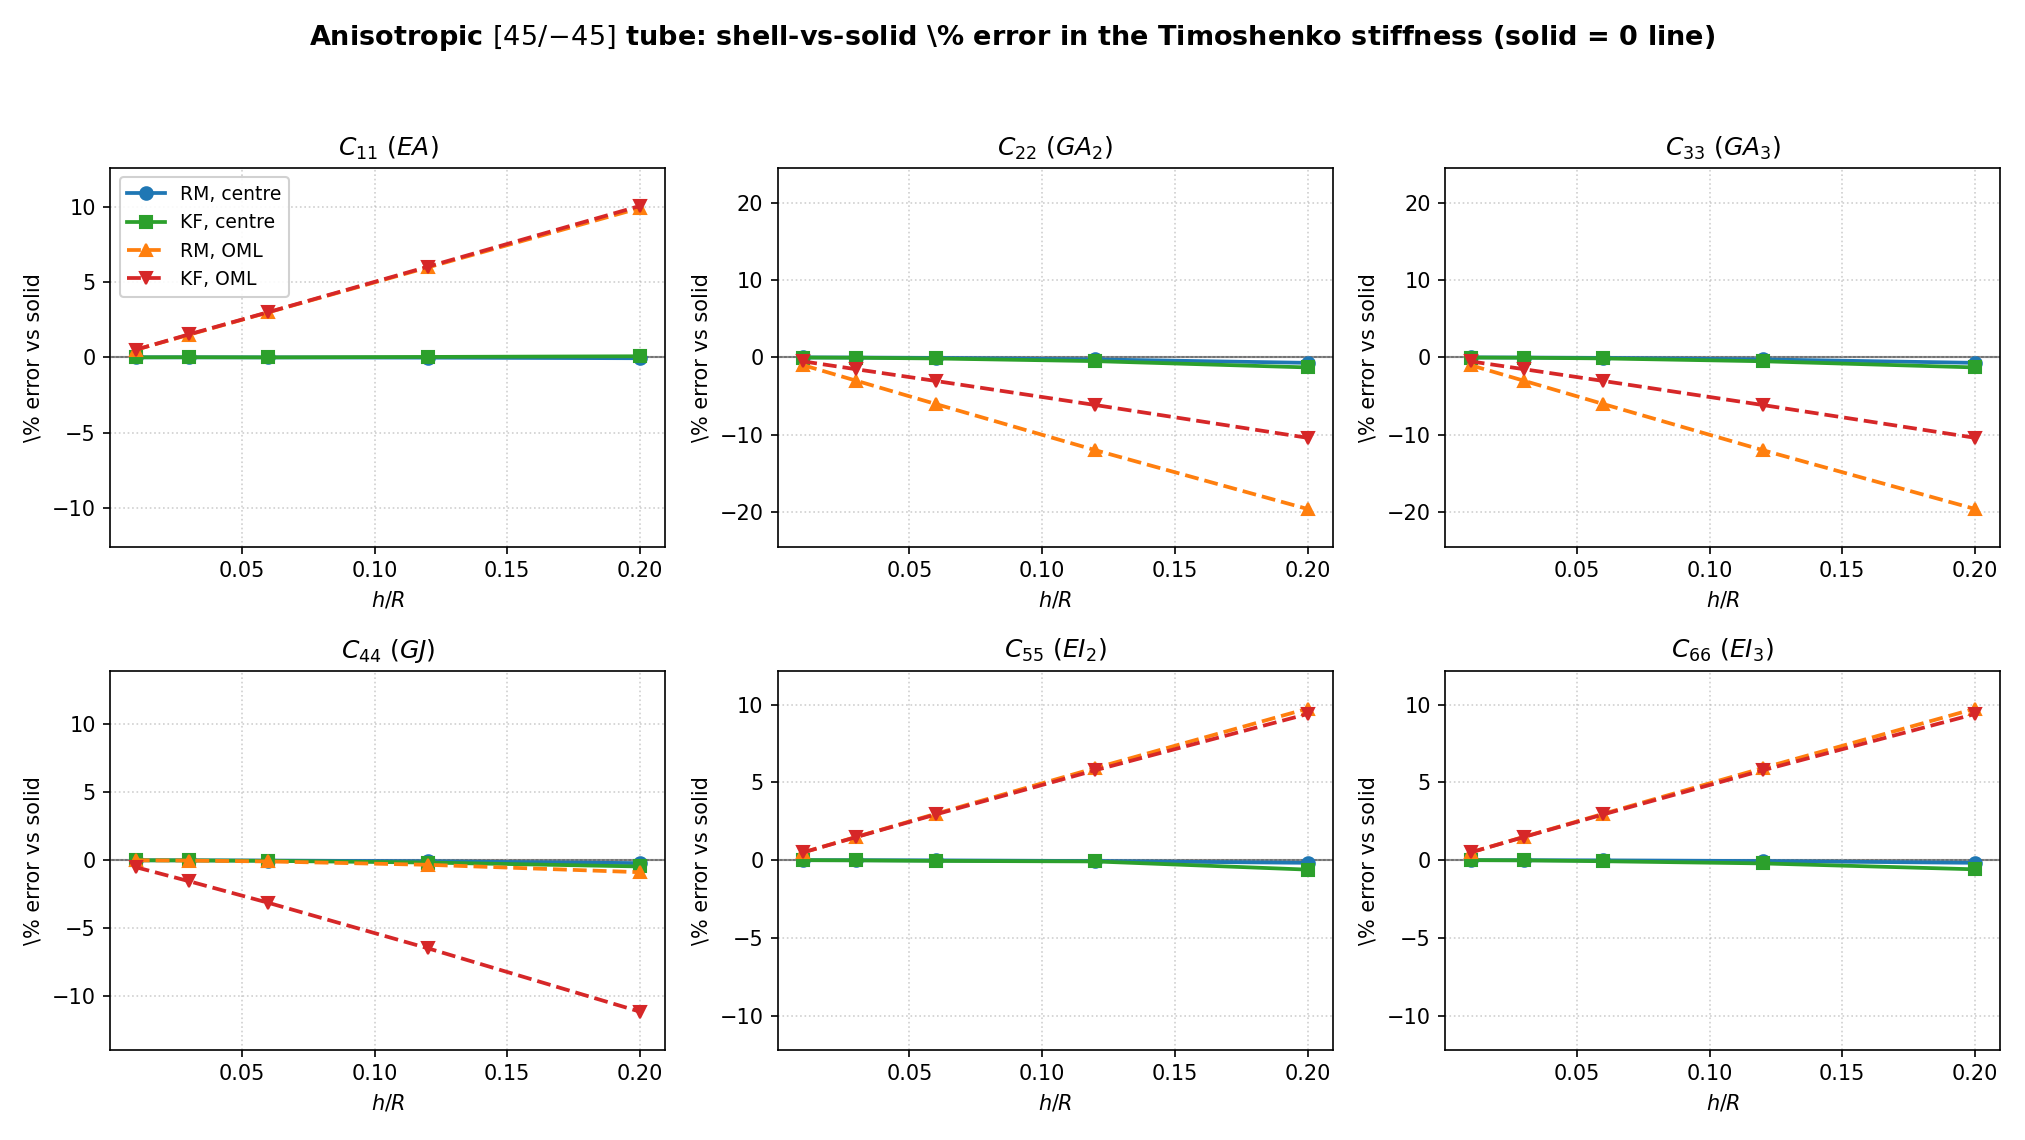
\includegraphics[width=0.96\textwidth]{err_tube_aniso.png}
\caption{Anisotropic $[45/\!-\!45]$ tube: \% error vs.\ the solid. Same behaviour
as the isotropic tube; $<1\%$ at the centre for both models across $h/R$.}
\label{fig:err_tube_aniso}
\end{figure}

\subsection{Flat plate-strip (open section)}
The open strip separates the stiffnesses into three groups
(Figs.~\ref{fig:err_strip_iso}--\ref{fig:err_strip_aniso};
Tables~\ref{tab:strip_iso_props}--\ref{tab:strip_aniso_full}).

\paragraph{Exact terms --- $EA$ and $EI_3$.} The axial stiffness and the strong
in-plane bending ($\sim W^3$) match the solid to $<2\%$ for both models, both
materials, across the whole range; the isotropic centre values equal the
Euler--Bernoulli closed form ($EA=EWh$, $EI_3=EhW^3/12$) exactly.

\paragraph{Torsion $GJ$ --- the open section corrects and vindicates RM.} For a
thin open strip the St-Venant constant is $J=Wh^3/3$. The closed tube hides the
torsion path because its $GJ$ is membrane (Bredt, $A_{66}$) dominated; the open
strip, having no closed cell, routes all of $GJ$ through the plate-twist measure.
This exposed a coefficient error in the RM twist row: the physical plate twist of
a beam twisting at rate $\kappa_1$ is $\kappa_{12}+\kappa_{21}=-2\kappa_1$, so the
macro must carry the full $-2$; a $-1$ split (relying on a rotation fluctuation
that a thin wall's transverse-shear stiffness locks to $\approx0$) under-counts
open-section torsion by exactly a factor of four ($Wh^3/3\!\to\!Wh^3/12$). With the
twist measure corrected to $-2$, the RM torsion is \emph{exact} ($GJ$ within
$0.2\%$ at the centre for all $h/W$) and the closed-tube $GJ$ is preserved
($-1.0\%\!\to\!-0.3\%$ at $h/R=0.20$). Kirchhoff, by contrast, over-stiffens the
open-section torsion as the wall thickens (\,$GJ$: $+0.5\%$ at $h/W=0.01$ rising to
$+22\%$ at $0.20$). The RM model is therefore the more accurate of the two for
thick open-section torsion (Fig.~\ref{fig:err_strip_iso}, panel $C_{44}$).

\paragraph{Weak bending $EI_2$ ($\sim h^3$).} At the centre this is captured by
both models; Kirchhoff is marginally better (within $-3$ to $+7\%$), while RM runs
slightly soft for $[45/\!-\!45]$ ($-10$ to $-20\%$), the expected effect of the
bend--twist coupling ($D_{16}\neq0$) on the free-warping cross-section. The OML
reference for $EI_2$ is dominated by the parallel-axis $EA\,(h/2)^2$ term and is a
pure reference offset, not a stiffness error (the OML curves run off-scale in the
plots; the values are in the tables).

\paragraph{Transverse shear $GA$ --- the method-sensitive group.} $GA_3$ (the
thickness-direction shear of a \emph{wide} strip) scales like $h^3$ and is a
genuinely two-dimensional field that a 1D-shell genome cannot represent; both RM
and Kirchhoff err on it ($-37\%$ thin to $+50$--$135\%$ thick), so it is a limit
of the shell idealization rather than of either kinematics. $GA_2$ (the in-plane
shear) is exact for the isotropic strip in both models; for the balanced
$[45/\!-\!45]$ strip Kirchhoff stays within $0$--$7\%$ while the RM $C^0$
kinematics under-predict it by $\approx33$--$46\%$. This RM residual is mesh- and
quadrature-converged (unchanged under full vs.\ selectively-reduced integration
and under doubling the genome resolution), i.e.\ it is intrinsic to the present RM
open-section shear-warping representation, not a discretization artifact, and
marks the open-section transverse-shear solve as the remaining item to refine.

\begin{figure}[t]\centering
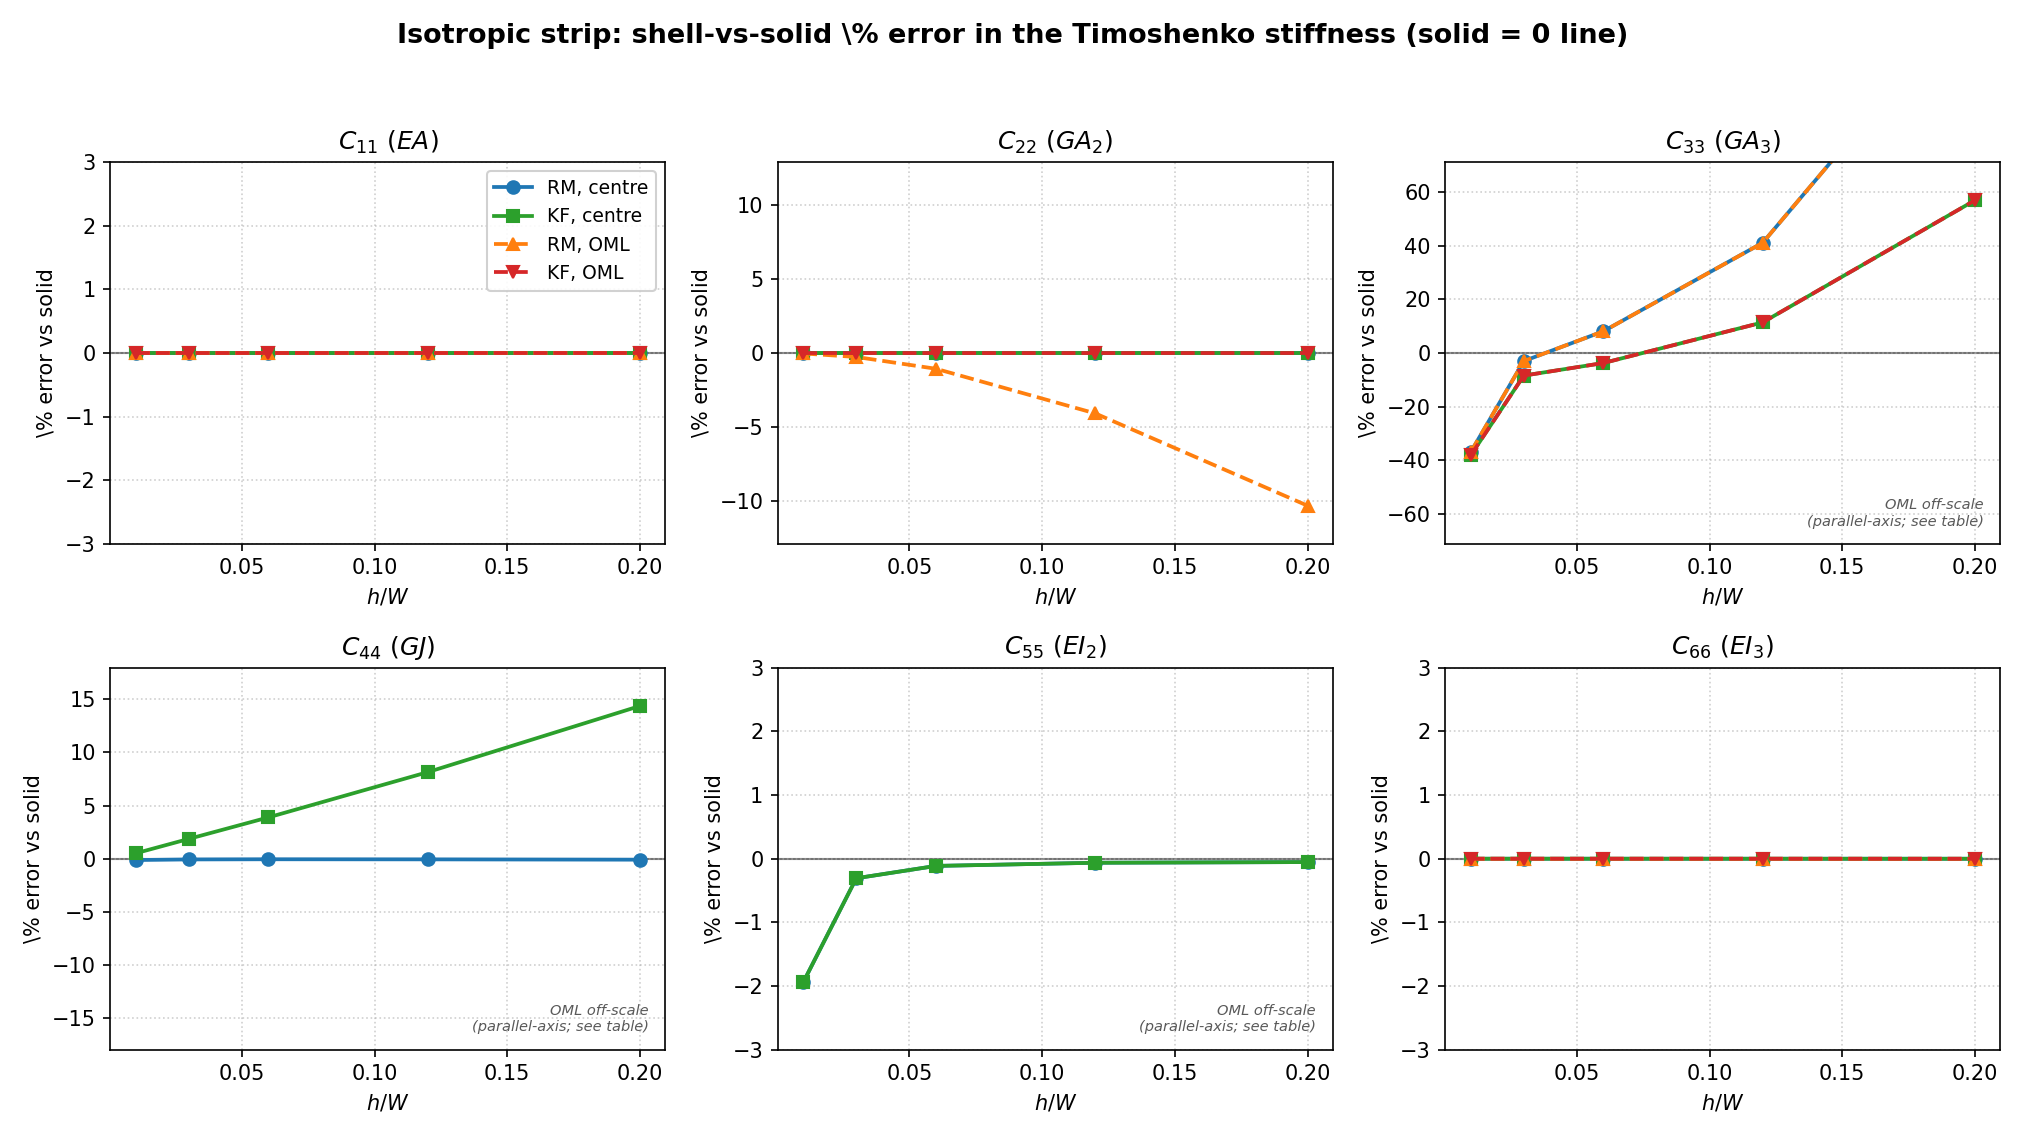
\includegraphics[width=0.96\textwidth]{err_strip_iso.png}
\caption{Isotropic strip: \% error vs.\ the solid. $EA$, $EI_3$ exact; $GJ$ exact
for RM and $+0.5$--$14\%$ for KF; $EI_2$ within $2\%$ for both; $GA_3$ off for
both (1D-shell limit). OML $EI_2$/$GJ$ are reference offsets (off-scale).}
\label{fig:err_strip_iso}
\end{figure}

\begin{figure}[t]\centering
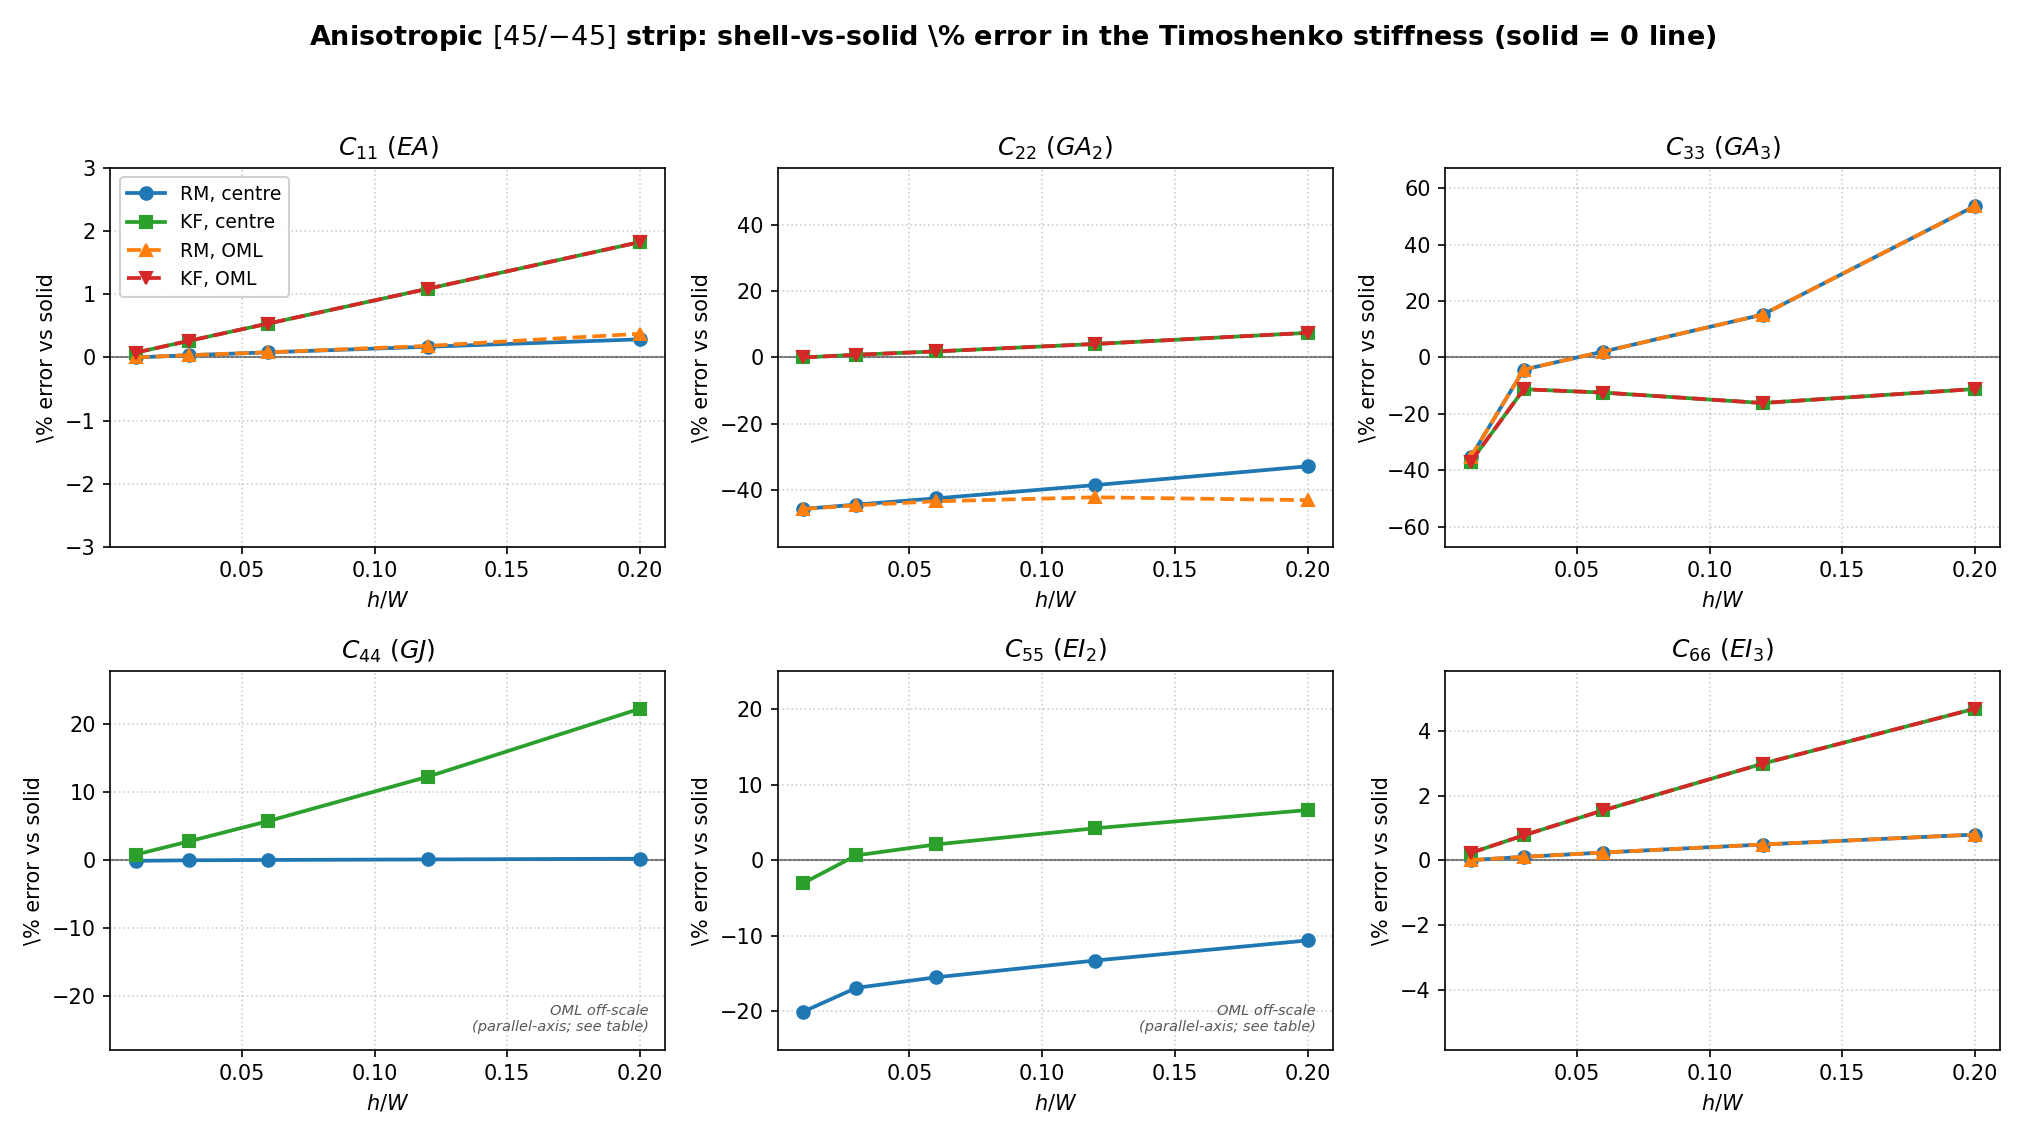
\includegraphics[width=0.96\textwidth]{err_strip_aniso.png}
\caption{Anisotropic $[45/\!-\!45]$ strip: \% error vs.\ the solid. $C_{44}$ ($GJ$):
RM exact, KF rising to $+22\%$. $C_{22}$ ($GA_2$): KF within $7\%$, RM $\approx-40\%$
(converged RM open-section residual). $C_{33}$ ($GA_3$): off for both (1D limit).
$C_{55}$ ($EI_2$): RM soft (bend--twist), KF closer.}
\label{fig:err_strip_aniso}
\end{figure}

\subsection{Coupling terms ($C_{14}$, $C_{15}$, $C_{16}$, $C_{25}$, $C_{36}$, $C_{56}$)}
Figs.~\ref{fig:coupl_tube_aniso}--\ref{fig:coupl_strip_iso} give the normalized
coupling coefficients $|c_{ij}|=|C_{ij}|/\sqrt{C_{ii}C_{jj}}$ (the off-diagonal
sign follows each model's axis convention---our solid and shell take opposite
through-thickness normals---so the convention-independent comparison is the
magnitude; the diagonal terms are sign-independent). Three facts organize the
results, and they are consistent with classical lamination theory and the
asymptotic thin-walled theory~\cite{deoyu2020,royyu2006,bagla2025}:

\begin{itemize}
\item \textbf{$C_{15}$ (ext--$M_2$), $C_{16}$ (ext--$M_3$), $C_{56}$ ($M_2$--$M_3$)
are \emph{identically zero} at the centroid} for both the circular and the
rectangular section, \emph{regardless of the $[45/\!-\!45]$ layup}: they require a
first moment ($C_{15},C_{16}$) or product of inertia ($C_{56}$) of the axial
stiffness about the reference axes, which vanishes for a stiffness distribution
symmetric about a centred circle / rectangle. In the data $C_{16},C_{56}$ sit at
the $10^{-13}$ floor. $C_{15}$ is zero at the centre and jumps to $\approx0.96$
\emph{only} at the OML reference---the textbook parallel-axis (Steiner) artifact
of an off-centroid reference line, not a material coupling.
\item \textbf{The genuine material couplings of the antisymmetric $[45/\!-\!45]$
section are $C_{14}$ (extension--twist, from $B_{16}$) and $C_{25}/C_{36}$
(transverse-shear--bending).} For the open strip they are large ($|c_{14}|\approx0.29$,
$|c_{25}|\approx0.43$); the centred shells reproduce $C_{14}$ well (both RM and KF
$\approx0.29$), and $C_{25}$ is captured by Kirchhoff ($\approx0.43$) but
under-predicted by RM ($\approx0.13$)---the same open-section shear-warping
residual seen in $GA_2$.
\item \textbf{The tube's couplings are an order of magnitude smaller}
($|c_{14}|,|c_{25}|,|c_{36}|\approx0.04$) because the closed wrap-around and the
circumferential averaging of the local $B$-coupling suppress what the flat open
strip expresses fully. All couplings vanish for the isotropic sections
(Figs.~\ref{fig:coupl_tube_iso},~\ref{fig:coupl_strip_iso}).
\end{itemize}

\begin{figure}[t]\centering
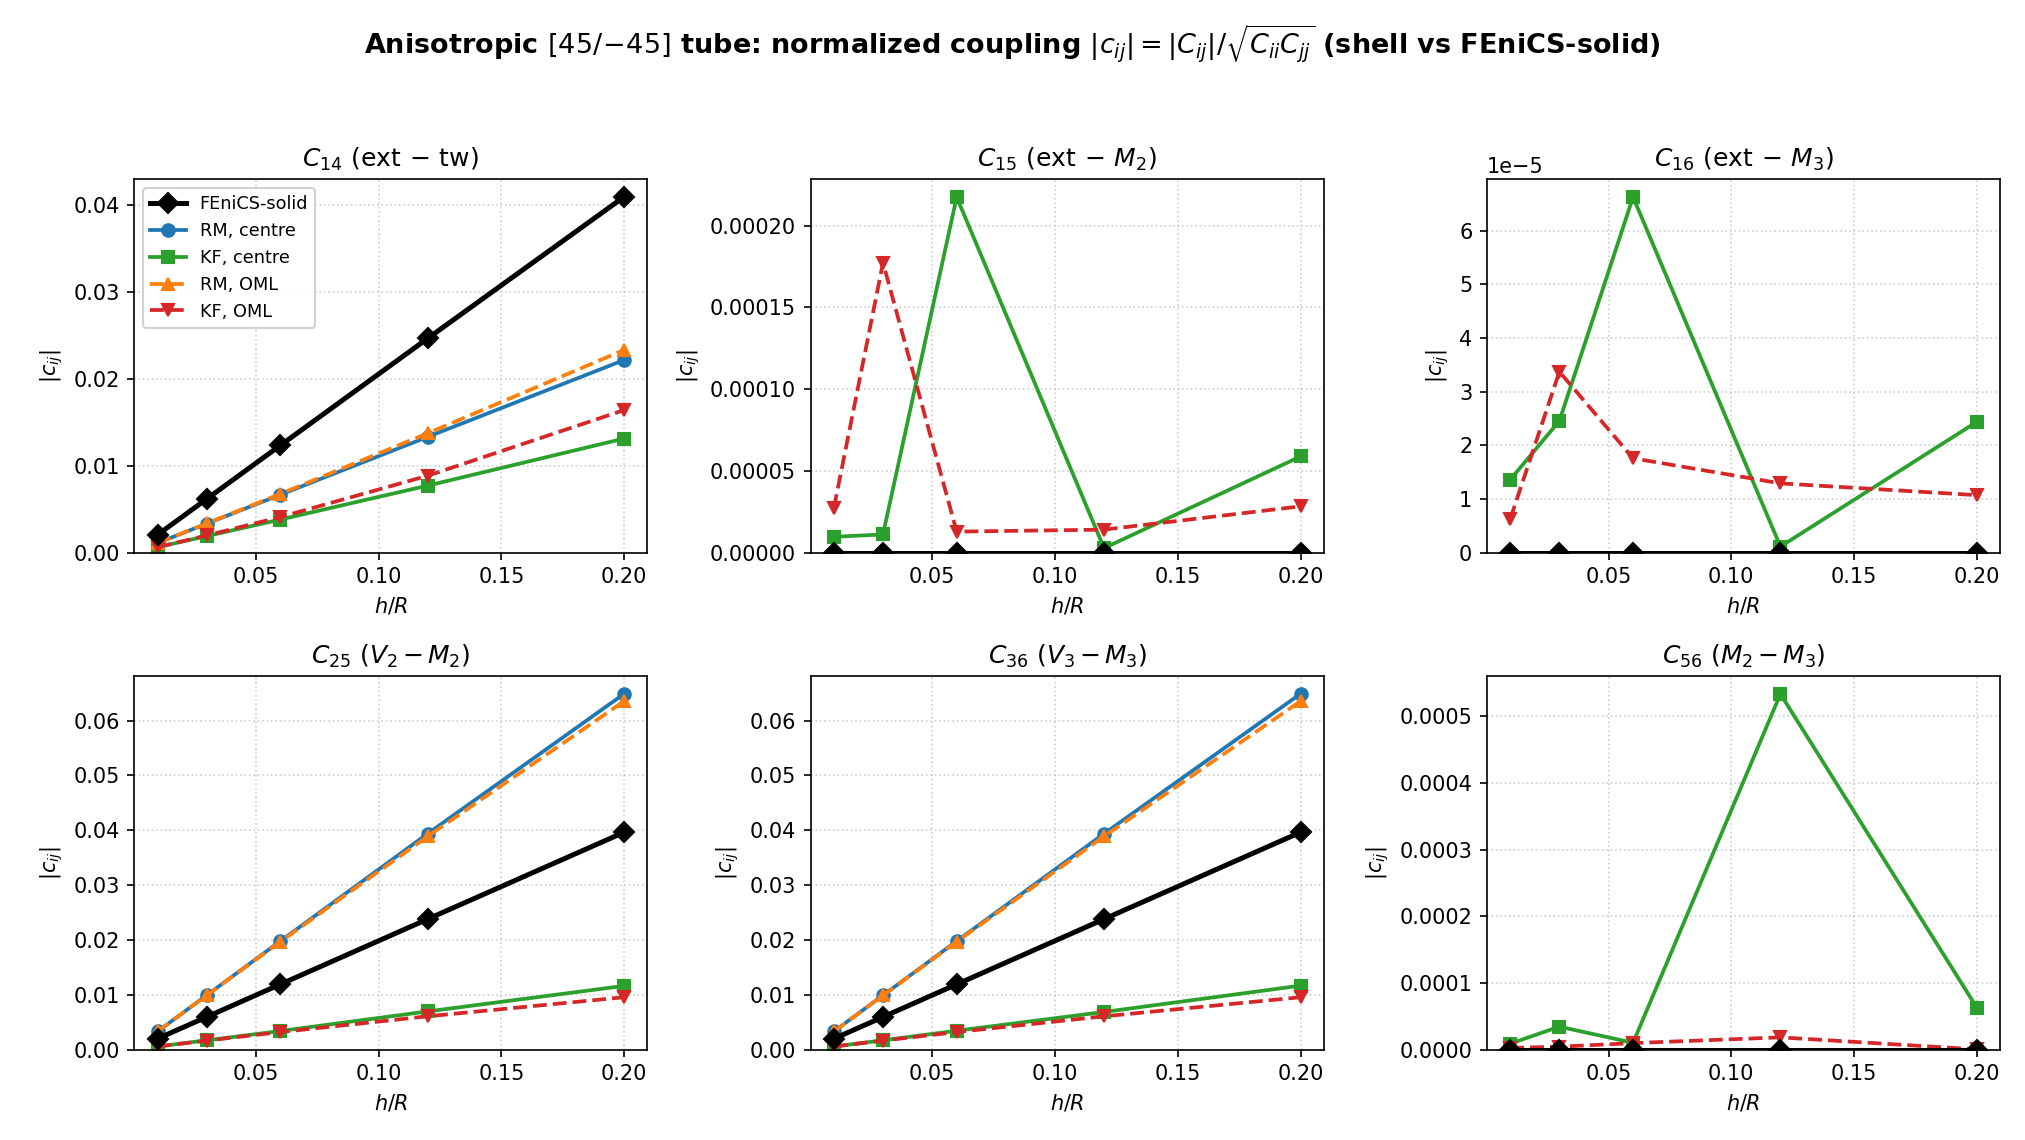
\includegraphics[width=0.96\textwidth]{coupl_tube_aniso.png}
\caption{Anisotropic $[45/\!-\!45]$ \textbf{tube}: normalized couplings vs.\ the
solid. Genuine $C_{14},C_{25},C_{36}\approx0.04$ (suppressed by closure);
$C_{15},C_{16},C_{56}\approx0$.}
\label{fig:coupl_tube_aniso}
\end{figure}

\begin{figure}[t]\centering
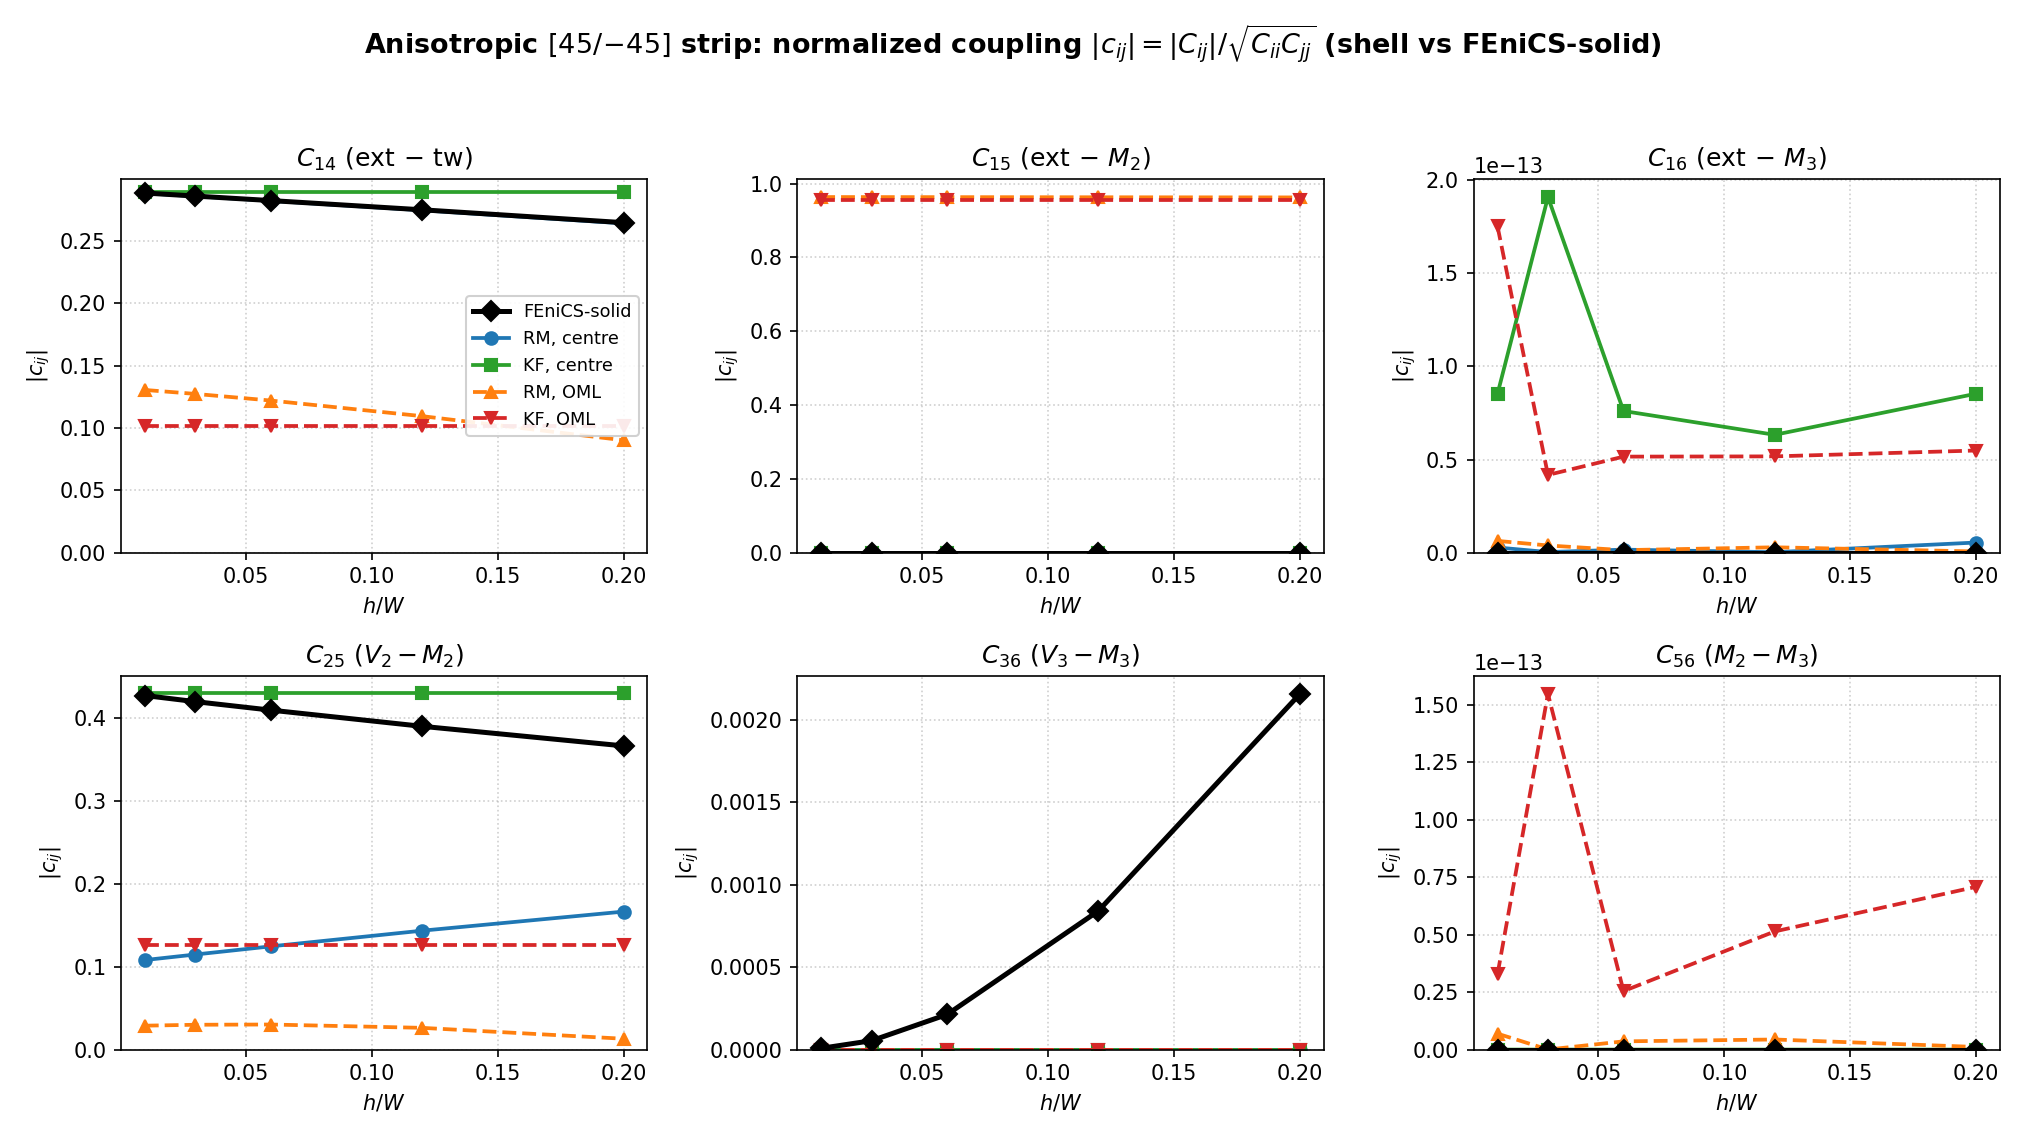
\includegraphics[width=0.96\textwidth]{coupl_strip_aniso.png}
\caption{Anisotropic $[45/\!-\!45]$ \textbf{strip}: $C_{14}$ ($\approx0.29$,
captured by both models) and $C_{25}$ ($\approx0.43$, captured by KF,
under-predicted by RM) are the genuine couplings; $C_{15}$ is the OML
parallel-axis artifact; $C_{16},C_{36},C_{56}\approx0$.}
\label{fig:coupl_strip_aniso}
\end{figure}

\begin{figure}[t]\centering
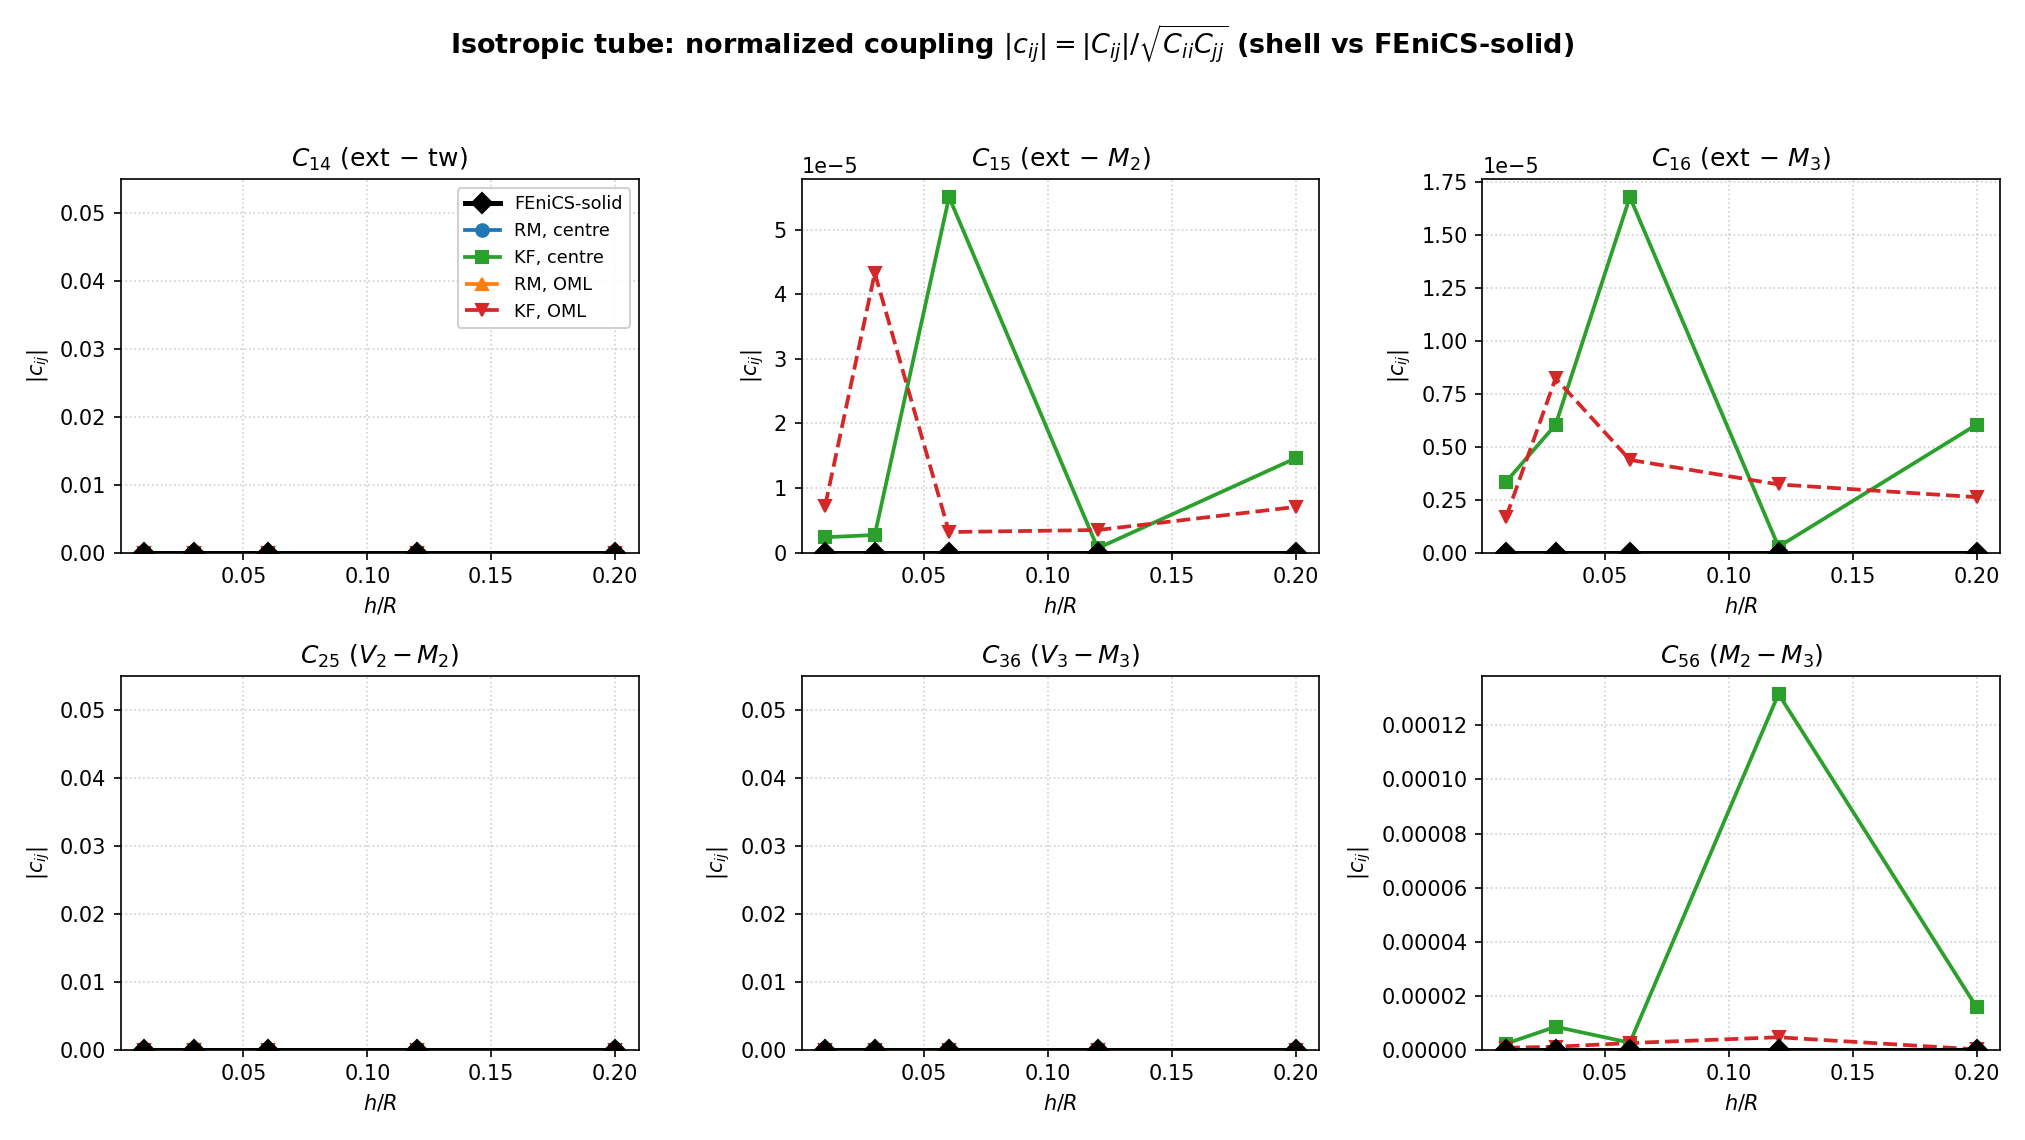
\includegraphics[width=0.49\textwidth]{coupl_tube_iso.png}\hfill
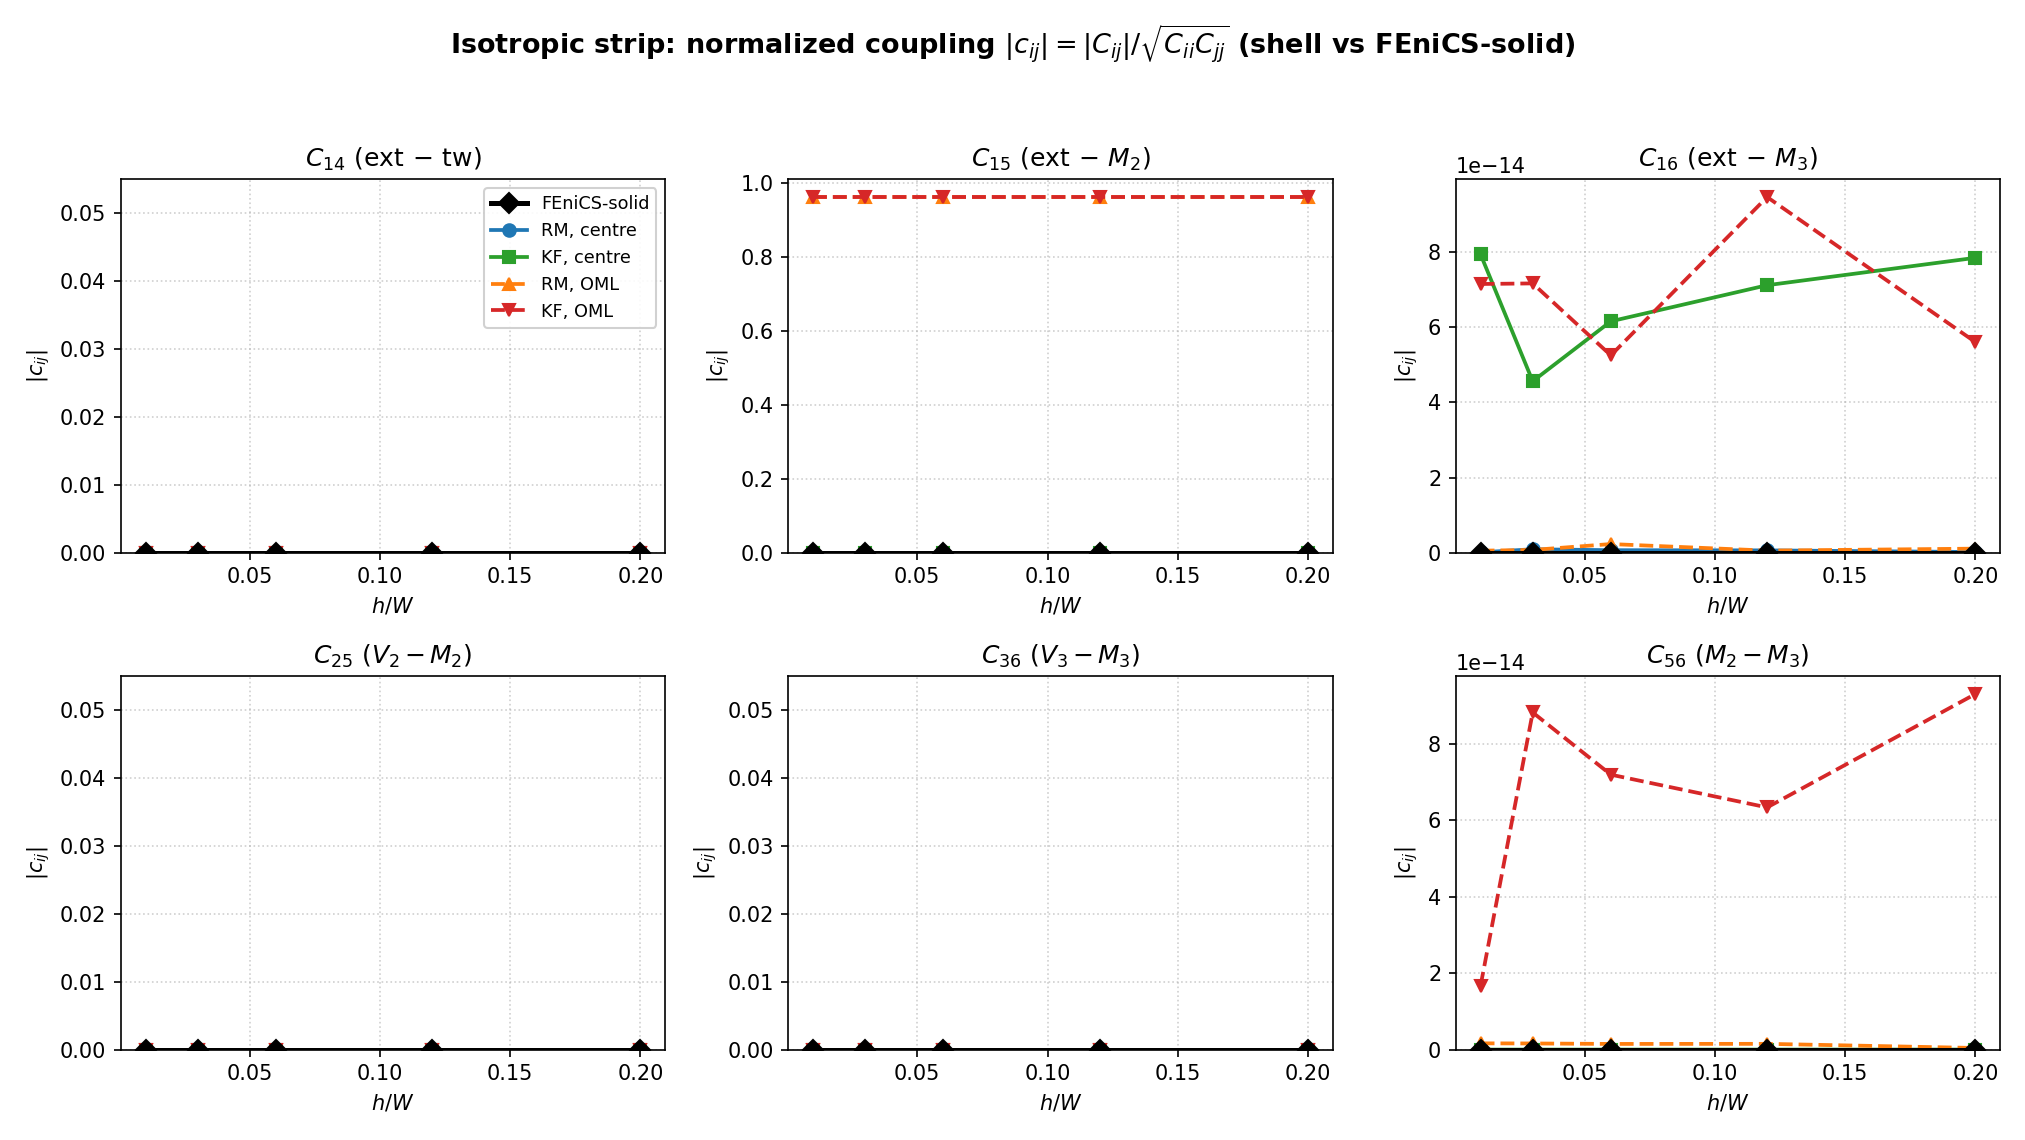
\includegraphics[width=0.49\textwidth]{coupl_strip_iso.png}
\caption{Isotropic tube (left) and strip (right): all material couplings vanish;
the only non-zero entry is the $C_{15}$ parallel-axis artifact at the OML
reference of the strip.}
\label{fig:coupl_strip_iso}
\end{figure}

% per-case Timoshenko tables (properties + thick-case error + full 6x6)
\begin{table}[t]\centering
\caption{Isotropic tube: EA vs $h/R$ (shell vs FEniCS-solid; \% relative to solid).}
\label{tab:iso_EA}
\begin{tabular}{lrrrrrr}\toprule
$h/R$ & solid & RM-ctr\% & KF-ctr\% & RM-OML\% & KF-OML\% & analytic\%\\\midrule
0.01 & 4.3975e+09 & +0.01 & +0.01 & +0.51 & +0.51 & +0.02\\
0.03 & 1.3193e+10 & +0.01 & +0.01 & +1.51 & +1.52 & +0.02\\
0.06 & 2.6385e+10 & +0.01 & +0.01 & +3.01 & +3.01 & +0.02\\
0.12 & 5.2770e+10 & +0.01 & +0.02 & +6.01 & +6.02 & +0.02\\
0.20 & 8.7950e+10 & +0.01 & +0.04 & +10.01 & +10.05 & +0.02\\
\bottomrule\end{tabular}\end{table}

\begin{table}[t]\centering
\caption{Isotropic tube: GA vs $h/R$ (shell vs FEniCS-solid; \% relative to solid).}
\label{tab:iso_GA}
\begin{tabular}{lrrrrrr}\toprule
$h/R$ & solid & RM-ctr\% & KF-ctr\% & RM-OML\% & KF-OML\% & analytic\%\\\midrule
0.01 & 8.4578e+08 & -0.00 & -0.01 & -1.00 & -0.51 & +0.00\\
0.03 & 2.5382e+09 & -0.02 & -0.03 & -2.97 & -1.51 & -0.03\\
0.06 & 5.0820e+09 & -0.07 & -0.11 & -5.88 & -3.02 & -0.14\\
0.12 & 1.0209e+10 & -0.28 & -0.39 & -11.51 & -6.03 & -0.58\\
0.20 & 1.7193e+10 & -0.76 & -1.05 & -18.59 & -10.06 & -1.61\\
\bottomrule\end{tabular}\end{table}

\begin{table}[t]\centering
\caption{Isotropic tube: GJ vs $h/R$ (shell vs FEniCS-solid; \% relative to solid).}
\label{tab:iso_GJ}
\begin{tabular}{lrrrrrr}\toprule
$h/R$ & solid & RM-ctr\% & KF-ctr\% & RM-OML\% & KF-OML\% & analytic\%\\\midrule
0.01 & 1.6911e+09 & -0.01 & -0.01 & +0.99 & -0.51 & +0.03\\
0.03 & 5.0743e+09 & -0.03 & -0.00 & +2.99 & -1.53 & +0.03\\
0.06 & 1.0156e+10 & -0.09 & +0.02 & +6.01 & -3.06 & +0.03\\
0.12 & 2.0366e+10 & -0.34 & +0.11 & +12.07 & -6.18 & +0.03\\
0.20 & 3.4160e+10 & -0.92 & +0.32 & +20.15 & -10.35 & +0.03\\
\bottomrule\end{tabular}\end{table}

\begin{table}[t]\centering
\caption{Isotropic tube: EI vs $h/R$ (shell vs FEniCS-solid; \% relative to solid).}
\label{tab:iso_EI}
\begin{tabular}{lrrrrrr}\toprule
$h/R$ & solid & RM-ctr\% & KF-ctr\% & RM-OML\% & KF-OML\% & analytic\%\\\midrule
0.01 & 2.1985e+09 & -0.00 & -0.00 & +0.50 & +0.50 & +0.03\\
0.03 & 6.5967e+09 & -0.01 & -0.01 & +1.49 & +1.49 & +0.03\\
0.06 & 1.3202e+10 & -0.05 & -0.06 & +2.95 & +2.94 & +0.03\\
0.12 & 2.6476e+10 & -0.19 & -0.19 & +5.79 & +5.76 & +0.03\\
0.20 & 4.4408e+10 & -0.53 & -0.63 & +9.39 & +9.32 & +0.03\\
\bottomrule\end{tabular}\end{table}

\begin{table}[t]\centering
\caption{Anisotropic [45/-45] tube: EA vs $h/R$ (shell vs FEniCS-solid; \% relative to solid).}
\label{tab:aniso_EA}
\begin{tabular}{lrrrrr}\toprule
$h/R$ & solid & RM-ctr\% & KF-ctr\% & RM-OML\% & KF-OML\%\\\midrule
0.01 & 7.7054e+08 & +0.01 & +0.01 & +0.51 & +0.51\\
0.03 & 2.3117e+09 & +0.01 & +0.01 & +1.51 & +1.53\\
0.06 & 4.6235e+09 & +0.00 & +0.00 & +3.00 & +3.02\\
0.12 & 9.2485e+09 & -0.01 & +0.04 & +5.99 & +6.04\\
0.20 & 1.5420e+10 & -0.05 & +0.08 & +9.94 & +10.08\\
\bottomrule\end{tabular}\end{table}

\begin{table}[t]\centering
\caption{Anisotropic [45/-45] tube: GA vs $h/R$ (shell vs FEniCS-solid; \% relative to solid).}
\label{tab:aniso_GA}
\begin{tabular}{lrrrrr}\toprule
$h/R$ & solid & RM-ctr\% & KF-ctr\% & RM-OML\% & KF-OML\%\\\midrule
0.01 & 3.2597e+08 & +0.00 & -0.01 & -1.00 & -0.51\\
0.03 & 9.7812e+08 & -0.01 & -0.04 & -3.00 & -1.52\\
0.06 & 1.9577e+09 & -0.06 & -0.13 & -6.02 & -3.04\\
0.12 & 3.9268e+09 & -0.25 & -0.47 & -11.96 & -6.14\\
0.20 & 6.5890e+09 & -0.69 & -1.29 & -19.56 & -10.37\\
\bottomrule\end{tabular}\end{table}

\begin{table}[t]\centering
\caption{Anisotropic [45/-45] tube: GJ vs $h/R$ (shell vs FEniCS-solid; \% relative to solid).}
\label{tab:aniso_GJ}
\begin{tabular}{lrrrrr}\toprule
$h/R$ & solid & RM-ctr\% & KF-ctr\% & RM-OML\% & KF-OML\%\\\midrule
0.01 & 6.5178e+08 & -0.01 & -0.01 & +0.99 & -0.51\\
0.03 & 1.9557e+09 & -0.02 & -0.02 & +3.00 & -1.54\\
0.06 & 3.9134e+09 & -0.07 & -0.05 & +6.03 & -3.13\\
0.12 & 7.8437e+09 & -0.27 & -0.17 & +12.15 & -6.47\\
0.20 & 1.3140e+10 & -0.73 & -0.46 & +20.37 & -11.13\\
\bottomrule\end{tabular}\end{table}

\begin{table}[t]\centering
\caption{Anisotropic [45/-45] tube: EI vs $h/R$ (shell vs FEniCS-solid; \% relative to solid).}
\label{tab:aniso_EI}
\begin{tabular}{lrrrrr}\toprule
$h/R$ & solid & RM-ctr\% & KF-ctr\% & RM-OML\% & KF-OML\%\\\midrule
0.01 & 3.8523e+08 & +0.00 & +0.00 & +0.50 & +0.50\\
0.03 & 1.1559e+09 & -0.00 & -0.01 & +1.50 & +1.49\\
0.06 & 2.3136e+09 & -0.01 & -0.05 & +2.99 & +2.95\\
0.12 & 4.6405e+09 & -0.06 & -0.08 & +5.93 & +5.78\\
0.20 & 7.7873e+09 & -0.17 & -0.61 & +9.75 & +9.40\\
\bottomrule\end{tabular}\end{table}

\begin{table}[t]\centering
\caption{Anisotropic [45/-45] tube: ext-twist vs $h/R$ (shell vs FEniCS-solid; \% relative to solid).}
\label{tab:aniso_exttwist}
\begin{tabular}{lrrrrr}\toprule
$h/R$ & solid & RM-ctr\% & KF-ctr\% & RM-OML\% & KF-OML\%\\\midrule
0.01 & 1.4575e+06 & -82.00 & -69.12 & -81.91 & -68.75\\
0.03 & 1.3118e+07 & -82.00 & -69.09 & -81.73 & -67.88\\
0.06 & 5.2466e+07 & -81.99 & -69.11 & -81.45 & -66.82\\
0.12 & 2.0980e+08 & -81.99 & -68.71 & -80.91 & -64.23\\
0.20 & 5.8239e+08 & -81.98 & -67.99 & -80.17 & -60.37\\
\bottomrule\end{tabular}\end{table}


\FloatBarrier
%================================================================
\section{Discussion and conclusions}
For \textbf{closed} thin-walled sections (the tube) the MSG shell is not merely a
thin-limit approximation: at the mid-surface reference it reproduces the full 3D
solid Timoshenko stiffness to $<1\%$ well into the thick regime ($h/R=0.20$), for
isotropic and balanced anisotropic walls, in both RM and Kirchhoff forms; the
dominant error for thick walls is the OML reference choice (an $O(h/R)$
curvature/arc-length bias), not the wall kinematics. The mid-surface reference is
recommended.

The \textbf{open} strip is the discriminating case. It cleanly separates terms the
shell captures exactly ($EA$, $EI_3$, and---with the corrected $-2$ twist
measure---$GJ$, where RM now matches St-Venant and beats Kirchhoff for thick
sections) from terms that are intrinsically harder: the weak bending $EI_2$
(bend--twist sensitive) and the transverse shear $GA$. Of the latter, the
thickness-direction $GA_3$ is a fundamental 1D-shell limitation shared by both
kinematics, whereas the in-plane $GA_2$ of the balanced strip is captured by
Kirchhoff but under-predicted by the present RM open-section shear-warping
representation---a converged, kinematic residual that is the natural target for
the next refinement. In short: use the mid-surface reference; trust $EA$, $EI$ and
(with the twist correction) $GJ$ in both models for open and closed sections; and
treat the open-section $GA$ as the method-sensitive quantity, with RM's standing
advantage being thick-section torsion and the recovery of transverse-shear stress
in dehomogenization (documented in the companion paper).

\paragraph{Reproducibility.}\begin{sloppypar}
The FEniCS 2D-solid cases (WSL) are generated by
\texttt{bench\_solid.py} and \texttt{bench\_strip\_solid.py}; the JAX MSG-TW shell
cases by \texttt{bench\_shell.py} and \texttt{bench\_strip\_shell.py}; the tables
and figures by \texttt{bench\_report.py}. Raw $6\times6$ data are in
\texttt{data/}. The twist-measure correction is at \texttt{rm/msg\_rm.py}
(\texttt{KAPPA12\_MACRO} $=-2$).\end{sloppypar}

%================================================================
% TODO: verify exact bibliographic details before distribution.
\begin{thebibliography}{9}
\bibitem{bagla2025} A.~Bagla, E.~Camarena, W.~Yu, Theory of arbitrarily-shaped
thin-walled composite beams via the mechanics of structure genome, Proc. American
Society for Composites (ASC), 2025.
\bibitem{royyu2006} M.~Roy, W.~Yu, Thin-walled composite beam cross-sectional
analysis, AIAA-2006-1647, 2006.
\bibitem{yu2012vabs} W.~Yu, D.~H. Hodges, J.~C. Ho, Variational asymptotic beam
sectional analysis --- an updated version, Int. J. Eng. Sci. 59 (2012) 40--64.
\bibitem{deoyu2020} A.~Deo, W.~Yu, Thin-walled composite beam cross-sectional
analysis using the mechanics of structure genome, Thin-Walled Structures 152 (2020).
\end{thebibliography}

\end{document}
